
%% bare_conf.tex
%% V1.4b
%% 2015/08/26
%% by Michael Shell
%% See:
%% http://www.michaelshell.org/
%% for current contact information.
%%
%% This is a skeleton file demonstrating the use of IEEEtran.cls
%% (requires IEEEtran.cls version 1.8b or later) with an IEEE
%% conference paper.
%%
%% Support sites:
%% http://www.michaelshell.org/tex/ieeetran/
%% http://www.ctan.org/pkg/ieeetran
%% and
%% http://www.ieee.org/

%%*************************************************************************
%% Legal Notice:
%% This code is offered as-is without any warranty either expressed or
%% implied; without even the implied warranty of MERCHANTABILITY or
%% FITNESS FOR A PARTICULAR PURPOSE! 
%% User assumes all risk.
%% In no event shall the IEEE or any contributor to this code be liable for
%% any damages or losses, including, but not limited to, incidental,
%% consequential, or any other damages, resulting from the use or misuse
%% of any information contained here.
%%
%% All comments are the opinions of their respective authors and are not
%% necessarily endorsed by the IEEE.
%%
%% This work is distributed under the LaTeX Project Public License (LPPL)
%% ( http://www.latex-project.org/ ) version 1.3, and may be freely used,
%% distributed and modified. A copy of the LPPL, version 1.3, is included
%% in the base LaTeX documentation of all distributions of LaTeX released
%% 2003/12/01 or later.
%% Retain all contribution notices and credits.
%% ** Modified files should be clearly indicated as such, including  **
%% ** renaming them and changing author support contact information. **
%%*************************************************************************


% *** Authors should verify (and, if needed, correct) their LaTeX system  ***
% *** with the testflow diagnostic prior to trusting their LaTeX platform ***
% *** with production work. The IEEE's font choices and paper sizes can   ***
% *** trigger bugs that do not appear when using other class files.       ***                          ***
% The testflow support page is at:
% http://www.michaelshell.org/tex/testflow/



\documentclass[conference]{IEEEtran}
% Some Computer Society conferences also require the compsoc mode option,
% but others use the standard conference format.
%
% If IEEEtran.cls has not been installed into the LaTeX system files,
% manually specify the path to it like:
% \documentclass[conference]{../sty/IEEEtran}





% Some very useful LaTeX packages include:
% (uncomment the ones you want to load)


% *** MISC UTILITY PACKAGES ***
%
%\usepackage{ifpdf}
% Heiko Oberdiek's ifpdf.sty is very useful if you need conditional
% compilation based on whether the output is pdf or dvi.
% usage:
% \ifpdf
%   % pdf code
% \else
%   % dvi code
% \fi
% The latest version of ifpdf.sty can be obtained from:
% http://www.ctan.org/pkg/ifpdf
% Also, note that IEEEtran.cls V1.7 and later provides a builtin
% \ifCLASSINFOpdf conditional that works the same way.
% When switching from latex to pdflatex and vice-versa, the compiler may
% have to be run twice to clear warning/error messages.






% *** CITATION PACKAGES ***
%
\usepackage{cite}
% cite.sty was written by Donald Arseneau
% V1.6 and later of IEEEtran pre-defines the format of the cite.sty package
% \cite{} output to follow that of the IEEE. Loading the cite package will
% result in citation numbers being automatically sorted and properly
% "compressed/ranged". e.g., [1], [9], [2], [7], [5], [6] without using
% cite.sty will become [1], [2], [5]--[7], [9] using cite.sty. cite.sty's
% \cite will automatically add leading space, if needed. Use cite.sty's
% noadjust option (cite.sty V3.8 and later) if you want to turn this off
% such as if a citation ever needs to be enclosed in parenthesis.
% cite.sty is already installed on most LaTeX systems. Be sure and use
% version 5.0 (2009-03-20) and later if using hyperref.sty.
% The latest version can be obtained at:
% http://www.ctan.org/pkg/cite
% The documentation is contained in the cite.sty file itself.






% *** GRAPHICS RELATED PACKAGES ***
%
\ifCLASSINFOpdf
   \usepackage[pdftex]{graphicx}
  % declare the path(s) where your graphic files are
   \graphicspath{{./images/}}
  % and their extensions so you won't have to specify these with
  % every instance of \includegraphics
   \DeclareGraphicsExtensions{.pdf}
\else
  % or other class option (dvipsone, dvipdf, if not using dvips). graphicx
  % will default to the driver specified in the system graphics.cfg if no
  % driver is specified.
  % \usepackage[dvips]{graphicx}
  % declare the path(s) where your graphic files are
  % \graphicspath{{../eps/}}
  % and their extensions so you won't have to specify these with
  % every instance of \includegraphics
  % \DeclareGraphicsExtensions{.eps}
\fi
% graphicx was written by David Carlisle and Sebastian Rahtz. It is
% required if you want graphics, photos, etc. graphicx.sty is already
% installed on most LaTeX systems. The latest version and documentation
% can be obtained at: 
% http://www.ctan.org/pkg/graphicx
% Another good source of documentation is "Using Imported Graphics in
% LaTeX2e" by Keith Reckdahl which can be found at:
% http://www.ctan.org/pkg/epslatex
%
% latex, and pdflatex in dvi mode, support graphics in encapsulated
% postscript (.eps) format. pdflatex in pdf mode supports graphics
% in .pdf, .jpeg, .png and .mps (metapost) formats. Users should ensure
% that all non-photo figures use a vector format (.eps, .pdf, .mps) and
% not a bitmapped formats (.jpeg, .png). The IEEE frowns on bitmapped formats
% which can result in "jaggedy"/blurry rendering of lines and letters as
% well as large increases in file sizes.
%
% You can find documentation about the pdfTeX application at:
% http://www.tug.org/applications/pdftex





% *** MATH PACKAGES ***
%
\usepackage{amsmath}
% A popular package from the American Mathematical Society that provides
% many useful and powerful commands for dealing with mathematics.
%
% Note that the amsmath package sets \interdisplaylinepenalty to 10000
% thus preventing page breaks from occurring within multiline equations. Use:
%\interdisplaylinepenalty=2500
% after loading amsmath to restore such page breaks as IEEEtran.cls normally
% does. amsmath.sty is already installed on most LaTeX systems. The latest
% version and documentation can be obtained at:
% http://www.ctan.org/pkg/amsmath

\usepackage{amssymb}



% *** SPECIALIZED LIST PACKAGES ***
%
%\usepackage{algorithmic}
% algorithmic.sty was written by Peter Williams and Rogerio Brito.
% This package provides an algorithmic environment fo describing algorithms.
% You can use the algorithmic environment in-text or within a figure
% environment to provide for a floating algorithm. Do NOT use the algorithm
% floating environment provided by algorithm.sty (by the same authors) or
% algorithm2e.sty (by Christophe Fiorio) as the IEEE does not use dedicated
% algorithm float types and packages that provide these will not provide
% correct IEEE style captions. The latest version and documentation of
% algorithmic.sty can be obtained at:
% http://www.ctan.org/pkg/algorithms
% Also of interest may be the (relatively newer and more customizable)
% algorithmicx.sty package by Szasz Janos:
% http://www.ctan.org/pkg/algorithmicx




% *** ALIGNMENT PACKAGES ***
%
%\usepackage{array}
% Frank Mittelbach's and David Carlisle's array.sty patches and improves
% the standard LaTeX2e array and tabular environments to provide better
% appearance and additional user controls. As the default LaTeX2e table
% generation code is lacking to the point of almost being broken with
% respect to the quality of the end results, all users are strongly
% advised to use an enhanced (at the very least that provided by array.sty)
% set of table tools. array.sty is already installed on most systems. The
% latest version and documentation can be obtained at:
% http://www.ctan.org/pkg/array


% IEEEtran contains the IEEEeqnarray family of commands that can be used to
% generate multiline equations as well as matrices, tables, etc., of high
% quality.




% *** SUBFIGURE PACKAGES ***
%\ifCLASSOPTIONcompsoc
%  \usepackage[caption=false,font=normalsize,labelfont=sf,textfont=sf]{subfig}
%\else
%  \usepackage[caption=false,font=footnotesize]{subfig}
%\fi
% subfig.sty, written by Steven Douglas Cochran, is the modern replacement
% for subfigure.sty, the latter of which is no longer maintained and is
% incompatible with some LaTeX packages including fixltx2e. However,
% subfig.sty requires and automatically loads Axel Sommerfeldt's caption.sty
% which will override IEEEtran.cls' handling of captions and this will result
% in non-IEEE style figure/table captions. To prevent this problem, be sure
% and invoke subfig.sty's "caption=false" package option (available since
% subfig.sty version 1.3, 2005/06/28) as this is will preserve IEEEtran.cls
% handling of captions.
% Note that the Computer Society format requires a larger sans serif font
% than the serif footnote size font used in traditional IEEE formatting
% and thus the need to invoke different subfig.sty package options depending
% on whether compsoc mode has been enabled.
%
% The latest version and documentation of subfig.sty can be obtained at:
% http://www.ctan.org/pkg/subfig




% *** FLOAT PACKAGES ***
%
%\usepackage{fixltx2e}
% fixltx2e, the successor to the earlier fix2col.sty, was written by
% Frank Mittelbach and David Carlisle. This package corrects a few problems
% in the LaTeX2e kernel, the most notable of which is that in current
% LaTeX2e releases, the ordering of single and double column floats is not
% guaranteed to be preserved. Thus, an unpatched LaTeX2e can allow a
% single column figure to be placed prior to an earlier double column
% figure.
% Be aware that LaTeX2e kernels dated 2015 and later have fixltx2e.sty's
% corrections already built into the system in which case a warning will
% be issued if an attempt is made to load fixltx2e.sty as it is no longer
% needed.
% The latest version and documentation can be found at:
% http://www.ctan.org/pkg/fixltx2e


%\usepackage{stfloats}
% stfloats.sty was written by Sigitas Tolusis. This package gives LaTeX2e
% the ability to do double column floats at the bottom of the page as well
% as the top. (e.g., "\begin{figure*}[!b]" is not normally possible in
% LaTeX2e). It also provides a command:
%\fnbelowfloat
% to enable the placement of footnotes below bottom floats (the standard
% LaTeX2e kernel puts them above bottom floats). This is an invasive package
% which rewrites many portions of the LaTeX2e float routines. It may not work
% with other packages that modify the LaTeX2e float routines. The latest
% version and documentation can be obtained at:
% http://www.ctan.org/pkg/stfloats
% Do not use the stfloats baselinefloat ability as the IEEE does not allow
% \baselineskip to stretch. Authors submitting work to the IEEE should note
% that the IEEE rarely uses double column equations and that authors should try
% to avoid such use. Do not be tempted to use the cuted.sty or midfloat.sty
% packages (also by Sigitas Tolusis) as the IEEE does not format its papers in
% such ways.
% Do not attempt to use stfloats with fixltx2e as they are incompatible.
% Instead, use Morten Hogholm'a dblfloatfix which combines the features
% of both fixltx2e and stfloats:
%
% \usepackage{dblfloatfix}
% The latest version can be found at:
% http://www.ctan.org/pkg/dblfloatfix




% *** PDF, URL AND HYPERLINK PACKAGES ***
%
%\usepackage{url}
% url.sty was written by Donald Arseneau. It provides better support for
% handling and breaking URLs. url.sty is already installed on most LaTeX
% systems. The latest version and documentation can be obtained at:
% http://www.ctan.org/pkg/url
% Basically, \url{my_url_here}.




% *** Do not adjust lengths that control margins, column widths, etc. ***
% *** Do not use packages that alter fonts (such as pslatex).         ***
% There should be no need to do such things with IEEEtran.cls V1.6 and later.
% (Unless specifically asked to do so by the journal or conference you plan
% to submit to, of course. )


% correct bad hyphenation here
\hyphenation{op-tical net-works semi-conduc-tor}

%------------------------Thilo Package Area-----------------------------
%Package for writing german letters
\usepackage[utf8]{inputenc}

%-----------------------------------------------------------------------
\begin{document}
%
% paper title
% Titles are generally capitalized except for words such as a, an, and, as,
% at, but, by, for, in, nor, of, on, or, the, to and up, which are usually
% not capitalized unless they are the first or last word of the title.
% Linebreaks \\ can be used within to get better formatting as desired.
% Do not put math or special symbols in the title.
\title{Describing the role of Artificial Neural Networks in Reinforcement Learning}


% author names and affiliations
% use a multiple column layout for up to three different
% affiliations
\author{\IEEEauthorblockN{Thilo Stegemann}
\IEEEauthorblockA{University of Applied Sciences\\Applied Computer Science\\
12459 Berlin, Wilhelminenhofstraße 75A\\
Email: t.stegemann@gmx.de}}

% conference papers do not typically use \thanks and this command
% is locked out in conference mode. If really needed, such as for
% the acknowledgment of grants, issue a \IEEEoverridecommandlockouts
% after \documentclass

% for over three affiliations, or if they all won't fit within the width
% of the page, use this alternative format:
% 
%\author{\IEEEauthorblockN{Michael Shell\IEEEauthorrefmark{1},
%Homer Simpson\IEEEauthorrefmark{2},
%James Kirk\IEEEauthorrefmark{3}, 
%Montgomery Scott\IEEEauthorrefmark{3} and
%Eldon Tyrell\IEEEauthorrefmark{4}}
%\IEEEauthorblockA{\IEEEauthorrefmark{1}School of Electrical and Computer Engineering\\
%Georgia Institute of Technology,
%Atlanta, Georgia 30332--0250\\ Email: see http://www.michaelshell.org/contact.html}
%\IEEEauthorblockA{\IEEEauthorrefmark{2}Twentieth Century Fox, Springfield, USA\\
%Email: homer@thesimpsons.com}
%\IEEEauthorblockA{\IEEEauthorrefmark{3}Starfleet Academy, San Francisco, California 96678-2391\\
%Telephone: (800) 555--1212, Fax: (888) 555--1212}
%\IEEEauthorblockA{\IEEEauthorrefmark{4}Tyrell Inc., 123 Replicant Street, Los Angeles, California 90210--4321}}




% use for special paper notices
%\IEEEspecialpapernotice{(Invited Paper)}




% make the title area
\maketitle

% As a general rule, do not put math, special symbols or citations
% in the abstract
\begin{abstract}
 TODO : Write an awesome abstract at the end!
\end{abstract}

% no keywords




% For peer review papers, you can put extra information on the cover
% page as needed:
% \ifCLASSOPTIONpeerreview
% \begin{center} \bfseries EDICS Category: 3-BBND \end{center}
% \fi
%
% For peerreview papers, this IEEEtran command inserts a page break and
% creates the second title. It will be ignored for other modes.
\IEEEpeerreviewmaketitle

% An example of a floating figure using the graphicx package.
% Note that \label must occur AFTER (or within) \caption.
% For figures, \caption should occur after the \includegraphics.
% Note that IEEEtran v1.7 and later has special internal code that
% is designed to preserve the operation of \label within \caption
% even when the captionsoff option is in effect. However, because
% of issues like this, it may be the safest practice to put all your
% \label just after \caption rather than within \caption{}.
%
% Reminder: the "draftcls" or "draftclsnofoot", not "draft", class
% option should be used if it is desired that the figures are to be
% displayed while in draft mode.
%
%\begin{figure}[!t]
%\centering
%\includegraphics[width=2.5in]{myfigure}
% where an .eps filename suffix will be assumed under latex, 
% and a .pdf suffix will be assumed for pdflatex; or what has been declared
% via \DeclareGraphicsExtensions.
%\caption{Simulation results for the network.}
%\label{fig_sim}
%\end{figure}

% Note that the IEEE typically puts floats only at the top, even when this
% results in a large percentage of a column being occupied by floats.


% An example of a double column floating figure using two subfigures.
% (The subfig.sty package must be loaded for this to work.)
% The subfigure \label commands are set within each subfloat command,
% and the \label for the overall figure must come after \caption.
% \hfil is used as a separator to get equal spacing.
% Watch out that the combined width of all the subfigures on a 
% line do not exceed the text width or a line break will occur.
%
%\begin{figure*}[!t]
%\centering
%\subfloat[Case I]{\includegraphics[width=2.5in]{box}%
%\label{fig_first_case}}
%\hfil
%\subfloat[Case II]{\includegraphics[width=2.5in]{box}%
%\label{fig_second_case}}
%\caption{Simulation results for the network.}
%\label{fig_sim}
%\end{figure*}
%
% Note that often IEEE papers with subfigures do not employ subfigure
% captions (using the optional argument to \subfloat[]), but instead will
% reference/describe all of them (a), (b), etc., within the main caption.
% Be aware that for subfig.sty to generate the (a), (b), etc., subfigure
% labels, the optional argument to \subfloat must be present. If a
% subcaption is not desired, just leave its contents blank,
% e.g., \subfloat[].


% An example of a floating table. Note that, for IEEE style tables, the
% \caption command should come BEFORE the table and, given that table
% captions serve much like titles, are usually capitalized except for words
% such as a, an, and, as, at, but, by, for, in, nor, of, on, or, the, to
% and up, which are usually not capitalized unless they are the first or
% last word of the caption. Table text will default to \footnotesize as
% the IEEE normally uses this smaller font for tables.
% The \label must come after \caption as always.
%
%\begin{table}[!t]
%% increase table row spacing, adjust to taste
%\renewcommand{\arraystretch}{1.3}
% if using array.sty, it might be a good idea to tweak the value of
% \extrarowheight as needed to properly center the text within the cells
%\caption{An Example of a Table}
%\label{table_example}
%\centering
%% Some packages, such as MDW tools, offer better commands for making tables
%% than the plain LaTeX2e tabular which is used here.
%\begin{tabular}{|c||c|}
%\hline
%One & Two\\
%\hline
%Three & Four\\
%\hline
%\end{tabular}
%\end{table}


% Note that the IEEE does not put floats in the very first column
% - or typically anywhere on the first page for that matter. Also,
% in-text middle ("here") positioning is typically not used, but it
% is allowed and encouraged for Computer Society conferences (but
% not Computer Society journals). Most IEEE journals/conferences use
% top floats exclusively. 
% Note that, LaTeX2e, unlike IEEE journals/conferences, places
% footnotes above bottom floats. This can be corrected via the
% \fnbelowfloat command of the stfloats package.

% conference papers do not normally have an appendix

% Introduction : Which question or which problem was investigated?
\section{Introduction}
Artificial Intelligence is a huge, rewarding, rising and complex research field. More and more people are interested in AI every day. Students, researchers, economics, engineers, CEO's and investors are highly encouraged to use, understand and/or improve AI technologies. At some point in time an AI newcomer will get to the problems of Reinforcement Learning (RL) and therefore to Artificial Neural Networks (ANN's). Andrew Ng. describes AI as the new upcomming electricity: AI will change many different industries and it will have a huge general impact in everyday life. 

% Related Work / State of the art / Literature Review
\section{Related Work}

\subsection{Asynchronous Methods for Deep Reinforcement Learning}
The scientists from Google DeepMind and Montreal Institute for Learning Algorithms introduced asynchronous deep learning algorithms \cite{DBLP:journals/corr/MnihBMGLHSK16}. These asynchronous algorithms are based on four standard reinforcement learning algorithms: One-step Q-learning, one-step Sarsa, n-step Q-learning and advantage actor-critic. The paper explains the background of reinforcement learning and how the asynchronous reinforcement learning methods works. The study was approved by an experiment in an Atari 2600 evaluation environment . All four asynchronous algorithms where tested within the test environment  . The Atari 2600 environment tests where used to compare the performance of the four algorithms. The main finding of this study is that all four asynchronous deep reinforcement learning algorithms are able to train neural network controllers on a variety of domains in a stable manner. In addition their results show that stable train ing of neural networks through reinforcement learning is possible with both value-based and policy-based methods, off-policy as well as on-policy methods, and in discrete as well as continuous domains. 

\subsection{Deep Reinforcement Learning with Double Q-Learning}
Aim of this paper is to determine if the recent DQN (Deep Q Network) algorithm, which combines Q-learning with a deep neural network, suffers from substantial overestimations in some games in the Atari 2600 domain \cite{DBLP:journals/corr/HasseltGS15}. Furthermore the Google DeepMind contributors point out how the Double Q-learning algorithm can be generalized to work with large-scale function approximation to successfully reduce the DQN overoptimism, resulting in more stable and reliable learning. Finally they propose a specific adaptation to the DQN algorithm and show that the resulting algorithm (Double DQN) not only reduces the observed overestimation, as they hypothesized, but that this also leads to much better performance on several Atari 2600 games.

\subsection{Human-level controll through deep reinforcement learning}
The paper is about how to reach human-level control through a deep Q-network, that can learn successful policies directly from high-dimensional sensory inputs using end-to-end reinforcement learning \cite{DRL:HumanLevelControl}. The deep Q-network agent (in reinforcement learning an agent is the executing learning algorithm) is tested on the challenging classic Atari 2600 game environment. The result of this test demonstrated that the deep Q-network agent, receiving only the pixels and the game score as inputs, was able to surpass the performance of all previous algorithms and achieve a level comparable to that of a professional human games tester across a set of 49 games, using the same algorithm, network architecture and hyperparameters. 


\subsection{Mastering the game of Go with deep neural networks and tree search}

The paper from Google concerns two different algorithm approaches for deep reinforcement learning \cite{DRL:Silver_2016}. The first approach uses 'value networks' to evaluate board positions and 'policy networks' to select moves. These deep neural networks are trained by a novel combination of supervised learning from human expert games and reinforcement learning from games of self-play. They proof through experiments that this deep RL algorithm approach is capable of playing Go at the level of state-of-the-art Monte Carlo tree search. The second deep RL approach is a new seach algorithm that combines Monte Carlo simulation with value and policy networks. They used this search algorithm inside the application AlphaGo and the application achieved a 99.8\% winning rate against other Go programs and it defeated the human European Go champion by 5 games to 0.

\subsection{Playing Atari with Deep Reinforcement Learning}
The paper from DeepMind Technologies is about a deep learning model to successfully learn control policies directly from high-dimensional sensory input using reinforcement learning \cite{mnih-atari-2013}. They defined the model as a convolutional neural network (CNN). This CNN is trained with a variant of Q-learning. Input of the CNN is row pixels and output is a value function estimating future rewards. They apply this deep learning model to seven Atari 2600 games from the Arcade Learning Environment, with no adjustment of the architecture or learning algorithm. Result of this experiment is that it outperforms all previous approaches on sex ot the games and surpasses a human expert on three of them. 

\section{Reinforcement Learning}
Reinforcement learning (RL) problems consider an agent-environment interaction framework. Basics of reinforcement learning are mentioned in \cite{DBLP:journals/corr/MnihBMGLHSK16, DBLP:journals/corr/HasseltGS15, DRL:HumanLevelControl, DRL:Silver_2016, mnih-atari-2013}. As an in depth guide for reinforcement learning see \cite{sutton_barto_98}. The following part is about summarizing those background RL introductions. The agent (implementation of the learning algorithm) will interact with the environment (a Markov Decision Process). The agent will get rewards and states from the environment and the environment will get actions from the agent. The agent tries to learn optimal behaviour through trial and error attempts. The agent wants to know which actions in which states get the most long-term reward and fit this knowledge into a policy representation. A few main problems of this RL framework are: 
\begin{itemize}
\item The agent only gets a numerical reward from the environment at the end of a decision-sequence. \\ $\sim$ \textit{Delayed Reward}
\item How should the reward be assigned to the different steps of a decision-sequence? \\ $\sim$ \textit{Credit Assignment Problem}
\item How to handle vast action- and state-spaces? \\ $\sim$ \textit{Generalization Problem}
\end{itemize}

A major goal of RL is to find a global optimal policy. A policy is a function which maps states to actions. This policy will additionally get a vector of parameters. The parameter-vector changes the policy output. This parametrisation of the policy function is called “function approximation” and Artificial Neural Networks are a really great approach for approximating a policy function. Combining ANN's with reinforcement learning algorithms have so far shown spectacular results e.g.: The Google DeepMind Team programmed an AI which plays Go (a very complex strategy board game) at human grandmaster level \cite{DRL:Silver_2016}. With this approximation the problem of vast action- and state-spaces can be solved. To optimise the parameter-vector methods  like “Monte-Carlo Policy Gradient” or “Actor-Critic Policy Gradient” are applied to objective functions. Applications like TD-Gammon by Gerald Tesauro proved that learning complex strategy games with Artificial Neural Networks is possible and promising.

\subsection{Q-learning}

\subsection{Actor-critic approaches}

\section{Convolutional Neural Networks}

A convolutional neural network (CNN) consists of layers. There are different kinds of layers: input layer, convolutional layer (CONV), rectified linear unit layer (RELU), pooling layer (POOL), fully connected layer (FC) and an output layer. Some of these layers can appear multiple times. For example CONV $\rightarrow$ RELU $\rightarrow$ CONV $\rightarrow$ RELU $\rightarrow$ POOL ... FC. In neural networks in general between the output and the input layers are hidden layers. If there is more then one hidden layer between input and output layer, then the neural network is called a deep neural network. To understand the Deep Q-networks it is helpful to first think about how those convolutional neural networks work in detail. 

\paragraph{The Input layer} can be high dimensional sensory data. Considering the Atari 2600 arcade gaming environment \cite{DBLP:journals/corr/MnihBMGLHSK16, DBLP:journals/corr/HasseltGS15, DRL:HumanLevelControl} the input is a video stream of pixels at different time steps. At time step $t$ a video signal reduces to just an image of pixels and the complete sequence of images at all time steps equals the video signal. There is still more then the raw pixels from the video stream like the score value at each time step \cite{DRL:HumanLevelControl}. In terms of reinforcement learning the score signal is a reward signal and the video stream at each time step describes the state in which the agent is in.

\paragraph{The convolution layer} is about shifting a fixed sized window (a filter) around the whole input image. The size of the filter should be about 3x3 or 5x5 pixels small. Each time the 3x3 filter is applied on an image position it outputs exact one value for that position. A filter can be a representation for edges, lines or other shapes. A combination of those low level filters results in more complex filters like an eye or an ear. Andrej Karpathy created a great visualisation of the computation inside the convolution layer see section "Convolution Demo" in \cite{KarpathyCNN}.

\begin{figure}[!t]
\centering
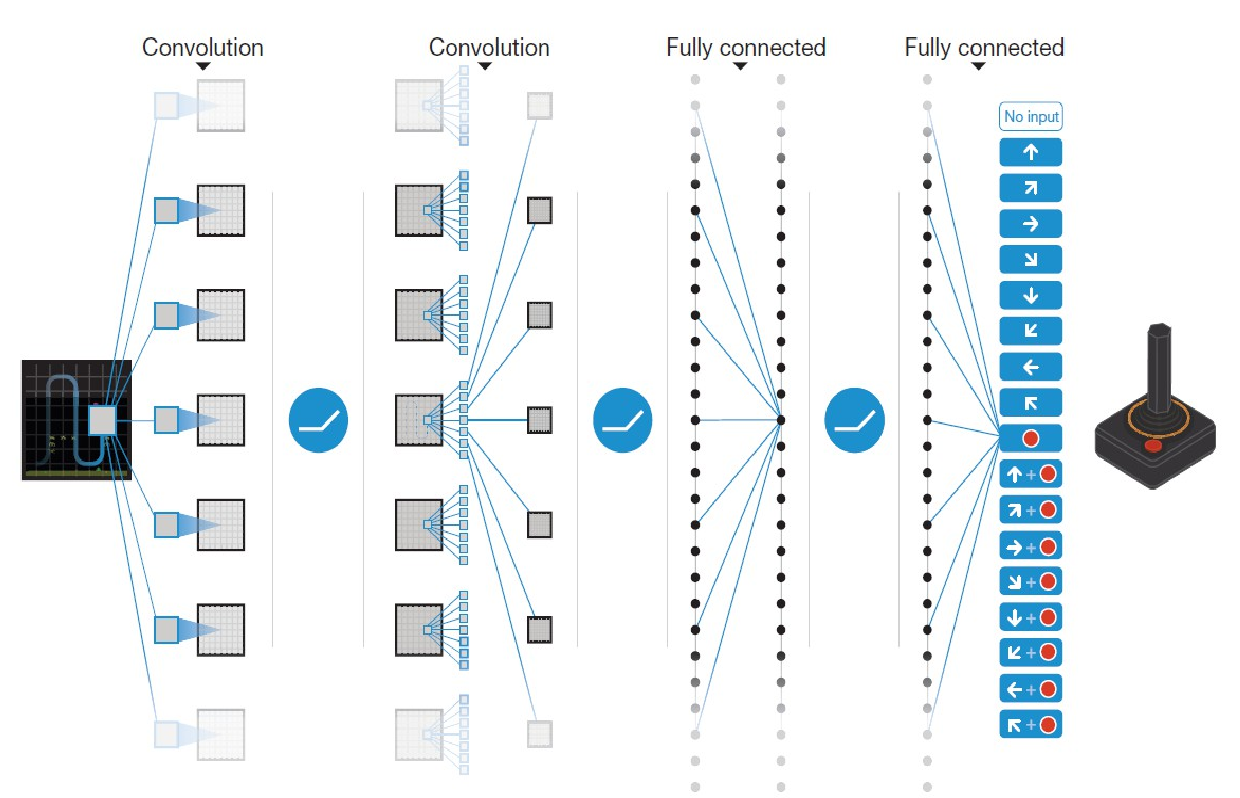
\includegraphics[width=3.5in]{conv_net}
\caption{Schematic illustration of the convolutional neural network \cite{DRL:HumanLevelControl}.}
\label{fig:conv_net}
\end{figure}

\section{Deep Q-network}
A deep Q network (DQN) is a combination of a convolutional neural network and the reinforcement learning algorithm Q-learning. 

"A deep Q network (DQN) is a multi-layerd neural network that for a given state $s$ outputs a vector of action values $Q(a, ; \theta)$, where $\theta$ are the parameters of the network. For an $n$-dimensional state space and an action space containing $m$ actions, the neural network is a function from $\mathbb{R}^n$ to $\mathbb{R}^m$. Two important ingredients of the DQN algorithm as proposed by Mnih et al. (2015) are the use of a target network and the use of experience replay. The target network, with parameters $\theta^-$, is the same as the online network except that its parameters are copied every $t$ steps from the online network, so that then $\theta^-_t = \theta_t$, and kept fixed on all other steps. The target used by DQN is then

\begin{equation*}
Y^{DQN}_t \equiv R_{t+1} + \gamma \max_a Q(S_{t+1}, a; \theta^-_t).
\end{equation*}

For the experience replay (Lin, 1992), observed transitions are stored for some time and sampled uniformly from this memory bank to update the network. Both the target network and the experience replay dramatically improve the performance of the algorithm (Mnih et al. 2015)."

% use section* for acknowledgment
% \section*{Acknowledgment}


%The authors would like to thank...





% trigger a \newpage just before the given reference
% number - used to balance the columns on the last page
% adjust value as needed - may need to be readjusted if
% the document is modified later
%\IEEEtriggeratref{8}
% The "triggered" command can be changed if desired:
%\IEEEtriggercmd{\enlargethispage{-5in}}

% references section

% can use a bibliography generated by BibTeX as a .bbl file
% BibTeX documentation can be easily obtained at:
% http://mirror.ctan.org/biblio/bibtex/contrib/doc/
% The IEEEtran BibTeX style support page is at:
% http://www.michaelshell.org/tex/ieeetran/bibtex/
\bibliographystyle{IEEEtran}
% argument is your BibTeX string definitions and bibliography database(s)
\bibliography{paper}
%
% <OR> manually copy in the resultant .bbl file
% set second argument of \begin to the number of references
% (used to reserve space for the reference number labels box)

% that's all folks
\end{document}


